\chapter{A brief tour of \mont}\label{chap:Monteverdi} 

\section{Introduction}\label{sec:montintro}
The \app package makes available a set of simple software
tools, which were designed to demonstrate what can be done with
\otb. Many users started using these applications for real processing
tasks, so we tried to make them more generic, more robust and easy to
use. \otb users have been asking for an integrated application for a
while, since using several applications for a complete processing
(ortho-rectification, segmentation, classification, etc.) can be a
burden. The OTB team received a request from CNES' Strategy
and Programs Office in order to provide an integrated application for
capacity building activities (teaching, simple image manipulation,
etc.). The specifications included ease of integration of new
processing modules.  


\section{Installation}\label{sec:montinstall}

The application is called \mont, since this is the name of the Orfeo
composer. The application allows you to build interactivelly remote
sensing processes based on the \otb. This is also in
remembering of the great (and once open source) Khoros/Cantata
software.
  
Installation of \mont is very simple. Standard installer packages are available on the main platforms thanks to OTB-Developpers and external users. 
These packages are available few days after the release. Get the latest information on binary packages on the \website in the section download.

We will discribe in the following sections the way to install \mont on:
\begin{itemize}
\item Windows platform (XP/Seven)
\item Ubuntu 14.X and higher
\item MacOSX 10.10
\end{itemize}

If you want to build from source or if we don't provide packages for your system, some informations are available into the \sg, in the section \textbf(Building from Source).
Note that the git repository of \mont is located here : https://git.orfeo-toolbox.org/monteverdi2.git.
In order to get the source of \mont, you will ahve te be placed on the right branch : git checkout 3.0.0-rc1


\subsection{Windows XP/Seven/8.1}
For Windows XP/Seven/8.1 users, there is a classical standalone installation program for \mont, available from the \download after each release. 

It is also possible to get \mont package through \osgeow for Windows XP/Seven users. 
Package for \mont is available directly in the OSGeo4W installer when you select the \textbf{otb-monteverdi} package. 
Follow the instructions in the OSGeo4W installer and select the \textbf{otb-monteverdi}. 
The installer will proceed with the installation of the package and all its dependencies. 
\mont will be directly installed in the OSGeo4W repository and a shortcut will be added to your desktop and in the start menu (in the OSGeo4W folder). 
You can now use directly \mont from your desktop, from the start menu and from an OSGeo4W shell with command \texttt{monteverdi}. 
Currently, you should use the 32bit OSGeo4W installer but we will soon distribute \mont package for 64 bit installer. 

\subsection{MacOS X}
A standard DMG package is available for \mont for MacOS X 10.10. Please go the \download.
Click on the file to launch \mont. 

\subsection{Ubuntu 14.x and higher}
For Ubuntu 14.x and higher, \mont package may be available as Debian package through APT repositories.

You can add it by using these command-lines:
\begin{verbatim}
sudo aptitude install add-apt-repository
sudo apt-add-repository ppa:ubuntugis/ubuntugis-unstable
\end{verbatim}

Now run:
\begin{verbatim}
sudo aptitude install monteverdi
\end{verbatim}

If you are using \emph{Synaptic}, you can add the repository, update and install the package through the
graphical interface.

\textbf{apt-add-repository} will try to retrieve the GPG keys of the
repositories to certify the origin of the packages. If you are behind a http
proxy, this step won't work and apt-add-repository will stall and eventually
quit. You can temporarily ignore this error and proceed with the update
step. Following this, aptitude update will issue a warning about a signature
problem. This warning won't prevent you from installing the packages.


\section{GUI : what does it look like ?}\label{sec:mongui}


\begin{figure}[!h] 
  \center
  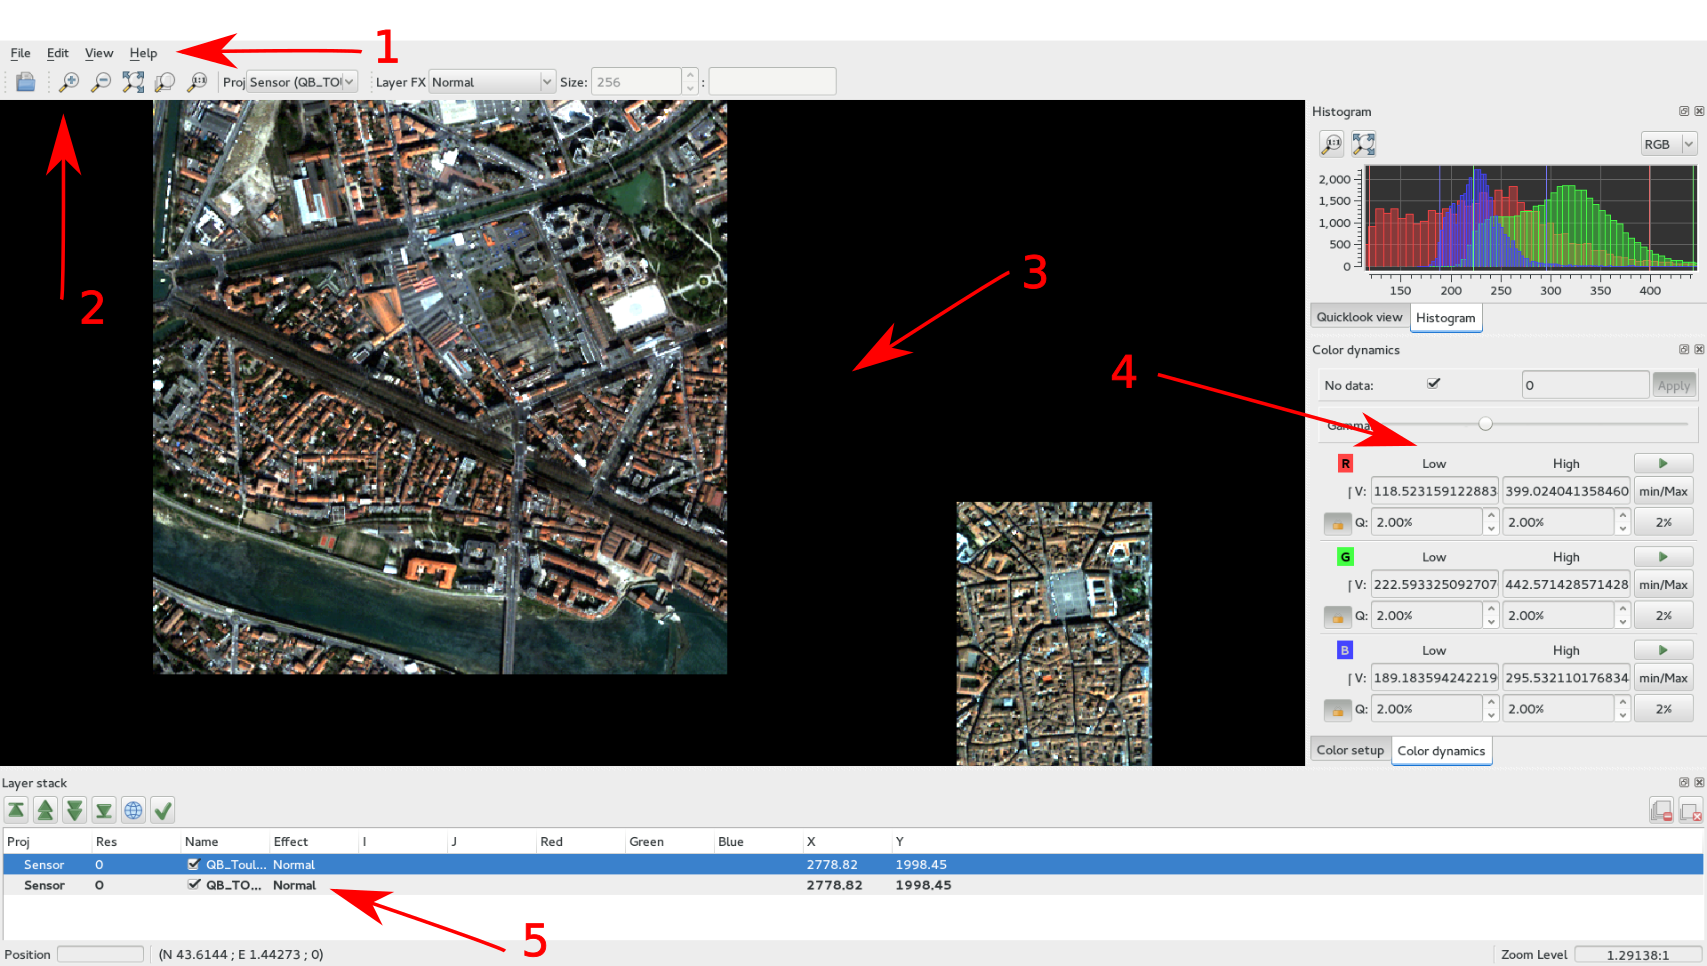
\includegraphics[width=0.95\textwidth]{../Art/MonteverdiImages/gui.png}
  \itkcaption[Monteverdi main window]{\mont's main window.}
  \label{fig:mongui}
\end{figure}

This is \mont's main window (figure ~\ref{fig:mongui}) where the
different functionalities are reachable:

\begin{itemize}
\item 1. Main menu
\item 2. Top toolbar
\item 3. Image displaying
\item 4. Right side dock
\item 5. Stack layer 
\end{itemize}

\subsection{Main menu}
The main menu is made up of four items.
The main one is the File item, from which you can : open a image, load the otb applications, and finally quit \mont.
The Edit item lets the user change his/her preferences. The view item is intended to let the user display or hide different parts of the main window.
Finally, the Help item lets the user know the 'About' information of the software, and also can display an useful keymap.

\subsection{Top toolbar}
The top toolbar is made up of ten icons; from left to right:
\begin{itemize}
\item 1st : open one or more image(s)
\item 2nd : zoom in
\item 3rd : zoom out
\item 4th : zoom to full extent
\item 5th : zoom to layer extent
\item 6th : zoom to full resolution
\item 7th : gives/changes the current projection, used as reference of the view 
\item 8th : selects the effect to be applied to the selected layer : chessboard, local constrast, local translucency, normal, spectral angle, swipe (horizontal and vertical)
\item 9th : a parameter used for the following effects : chessboard, local contrast, local translucency, spectral angle
\item 10th : a parameter used for the following effects :  local constrast, spectral angle
\end{itemize}

\subsection{Image displaying}
This part of the main window is intented to display the images loaded by the user.
There are many nice keyboard shortcuts or mouse tricks that let the user have a better experience in navigating throughout the loaded images.
These shortcuts and tricks are given within the Help item of the main menu, by clicking Keymap; here is a short list of the most useful ones :

The classical ones:
\begin{itemize}
\item CTRL+O = Open file(s)
\item CTRL+Q = Quit application
\end{itemize}

In the image displaying part:
\begin{itemize}
\item Mouse drag = Scroll view
\item CTRL+Mouse drag = Quick scroll view (rending is done after releasing CTRL key)
\item CTRL+Mouse wheel = Zoom in out
\item + or - = Zoom in out
\end{itemize}

In the layer stack part:
\begin{itemize}
\item SHIFT+Page Up = Move layer to top of stack
\item SHIFT+Page Down = Move layer to bottom of stack
\item Delete = Delete selected layer
\item SHIFT+Delete = Delete all layers
\end{itemize}


\subsection{Right side dock}
The dock on the right side is divided into four tabs : 
\begin{itemize}
\item Quicklook : gives the user a degraded view of the whole extent, letting him/her easily select the area to be displayed 
\item Histogram : gives the user information about the value distribution of the selected channels. By clicking the mouse's left button, user can sample their values.
\item Color Setup : lets the user map the image channels to the RGB channels. Also lets him/her set the alpha parameter (translucency).
\item Color dynamics : lets the user change the displaying dynamics of a selected image. For each RGB channel (each mapped to an image channel), the user can decide how the pixel range of a selected image will be shortcut before being rescaled to 0-255 : either by setting the extremal values, or by setting the extremal quantiles.
\end{itemize}

Each tab is represented by the figures below (~\ref{fig:quickhisto} ~\ref{fig:colorsetdyn}).

\begin{figure}[!h] 
  \center
  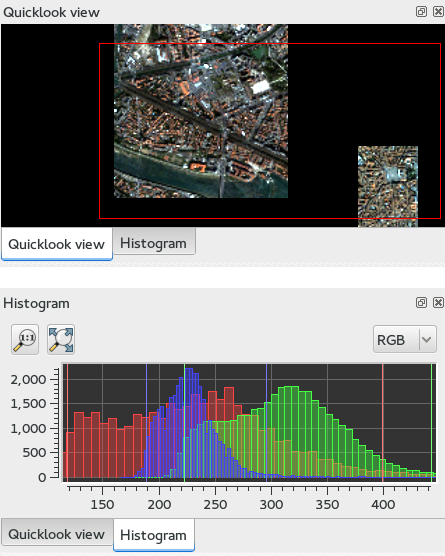
\includegraphics[width=0.8\textwidth]{../Art/MonteverdiImages/quickhisto.png}
  \itkcaption[Monteverdi quicklook tab]{Quicklook tab (op), histogram tab (bottom).}
  \label{fig:quickhisto}
\end{figure}

\begin{figure}[!h] 
  \center
  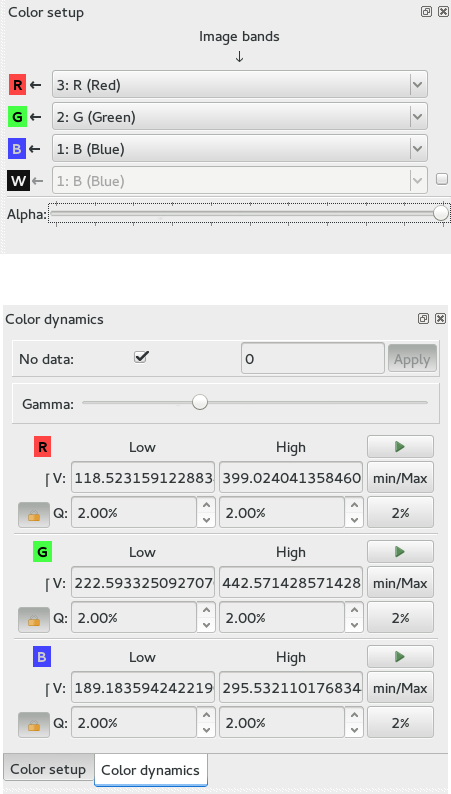
\includegraphics[width=0.66\textwidth]{../Art/MonteverdiImages/colsetdyn.png}
  \itkcaption[Monteverdi color setup tab]{Color setup tab (top), color dynamics tab (bottom).}
  \label{fig:colorsetdyn}
\end{figure}


\subsection{Layer stack}

The layer stack is made up of one list of layers located beneath six icons.
The list of layers gives the user some information about the loaded images:
projection, resolution (if available), name, and effect applied to the images (see top toolbar subsection).
If the user moves the mouse over the displayed images, he/she will get more information:

\begin{itemize}
\item (i,j) : pixel index
\item (Red Green Blue) : original image pixel values from channel mapped to the RGB ones.
\item (X,Y) : pixel position
\end{itemize}

Concerning the six icons, from left to right:
\begin{itemize}
\item 1st : moves the selected layer to the top of the stack
\item 2nd : moves the selected layer up within the stack
\item 3rd : moves the selected layer down within the stack
\item 4th : moves the selected layer to the bottom of the stack
\item 5th : use selected layer as projection reference
\item 6th : applies all display settings (color-setup, color-dynamics, shader and so forth) of selected layer to all other layers
\end{itemize}

The layer stack is represented in the figure below (~\ref{fig:layerstack}) :
\begin{figure}[!h] 
  \center
  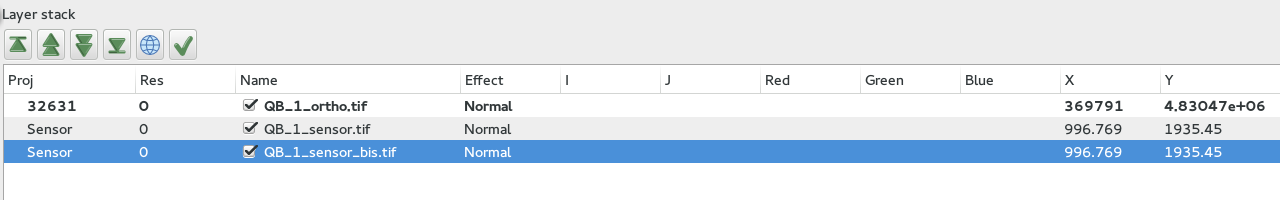
\includegraphics[width=0.95\textwidth]{../Art/MonteverdiImages/layerstack.png}
  \itkcaption[Monteverdi layerstack]{Layer stack.}
  \label{fig:layerstack}
\end{figure}


\section{Examples}\label{sec:monexamples}

With \mont, it is also possible to interactively load otb-applications and use them to process images.
For that purpose, the user just has to load otb-applications by clicking on the Main menu, File/Load OTB-Applications (or by simply using the shorcut CTRL+A).
The figure below (~\ref{fig:applications}) represents the otb-applications loading window. The applications are arranged in thematic functionalities; the user can also quickly find the wanted application by typing its name in the dedicated field
at the top of the loading window.


\begin{figure}[!h] 
  \center
  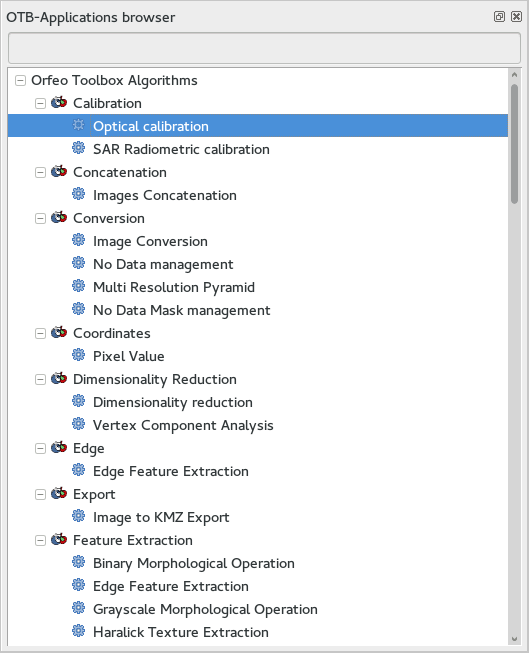
\includegraphics[width=0.6\textwidth]{../Art/MonteverdiImages/applications.png}
  \itkcaption[Monteverdi app]{Applications window.}
  \label{fig:applications}
\end{figure}


\subsection{Optical calibration}\label{ssec:monoptical}

In order to perform an optical calibration, launch the Optical calibration application (shortcut CTRL+A). 
We are going to use this application to perform a TOA (Top Of Atmosphere) conversion, which consists in converting the DN pixel values into spectral radiance (in W/m2/steradians/micrometers).
Once the application is launched, the user must fill the required fields in
(in, out, gainbias.txt -gain and bias values in a txt file-, solarillumination.txt -solar illumination values in watt/m2/micron for each band in a txt file-, and so on... refer to the documentation of the application).
\begin{itemize}
\item Note : if OTB (on which is based \mont) is able to parse the metadata of the image to be calibrated, then some of the fields will be automatically filled in.
\end{itemize}

In the figure below (~\ref{fig:OC}), by taking a look at the layer stack, one can notice that the values of the calibrated image are now expressed in spectral radiance.


\begin{figure}[!h] 
  \center
  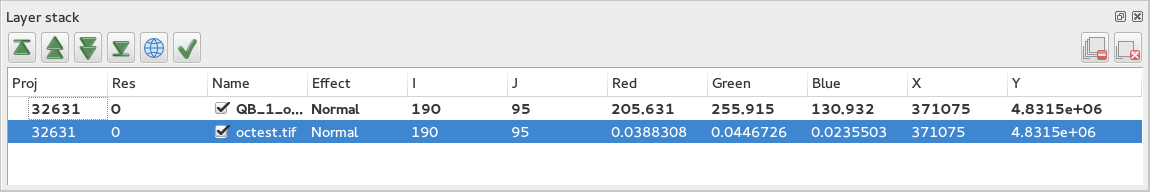
\includegraphics[width=0.95\textwidth]{../Art/MonteverdiImages/OC.png}
  \itkcaption[Monteverdi OC]{Before and after calibration.}
  \label{fig:OC}
\end{figure}



\subsection{BandMath}\label{ssec:monbandmath}

BandMath application is intented to apply mathematical operations on pixels (launch it with shortcut CTRL+A). In this example, we are going to use this application to change the dynamics of an image,
and check the result by looking at histogram tab, in the right side dock. The formula used is the following : im1b1*1000.
In the figures below (~\ref{fig:BM}), one can notice that the mode of the distribution is located at position 356.0935, whereas in the transformed image,
the mode is located at position 354737.1454, that's to say 1000 times farther away approximatelly (the cursors weren't placed exactly at the same position during screenshots).


\begin{figure}[!h] 
  \center
  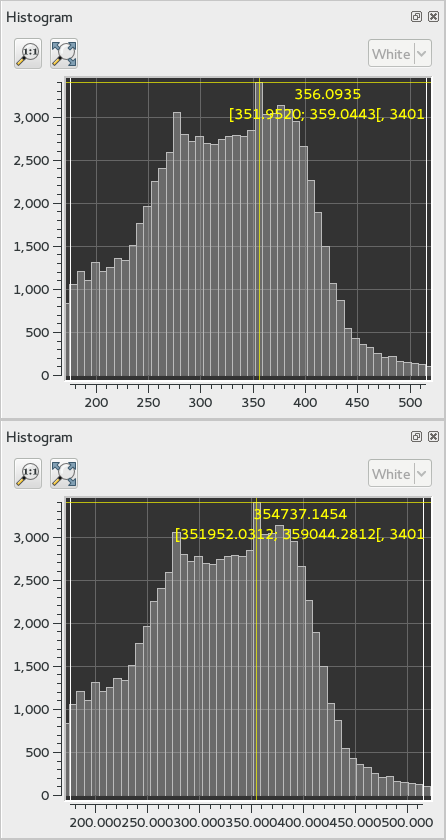
\includegraphics[width=0.5\textwidth]{../Art/MonteverdiImages/BM.png}
  \itkcaption[Monteverdi BM1]{Before/after applying BandMath (top/bottom).}
  \label{fig:BM}
\end{figure}


\subsection{Segmentation}\label{ssec:monseg}

Now, let's use the segmentation application (launch it with shortcut CTRL+A). 
We let the user take a look at the application's documentation; let's simply say that as we wish we could display the segmentation with \mont,
we must tell the application to output the segmentation in raster format. Thus, the value of the mode option must be set to raster.
The following figure (~\ref{fig:seg12}) shows the original image and the labels image.

\begin{figure}[!h] 
  \center
  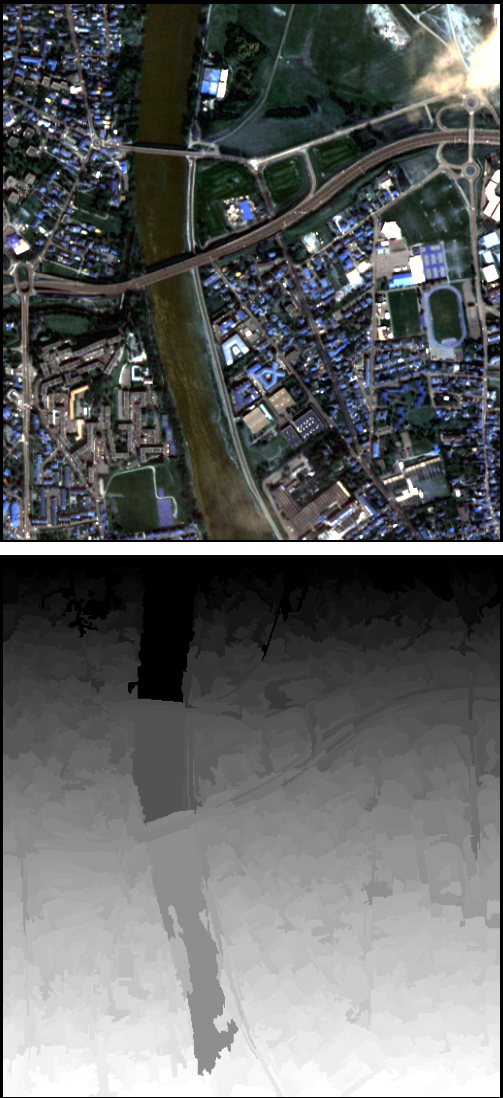
\includegraphics[width=0.45\textwidth]{../Art/MonteverdiImages/seg1-2.png}
  \itkcaption[Monteverdi seg12]{Original image and labels image.}
  \label{fig:seg12}
\end{figure}


Gray colors aren't very convenient for visualizing a segmentation. That's why we are going to use another application, the ColorMapping one (launch it with the sortcut CTRL+A as usual).
There are many ways to use this application (see the documentation for more details). We wish we could colour the segmentation so that color difference between adjacent regions is maximized.
For this purpose, we can use the method optimal (set the value of this option to optimal). The figure below (~\ref{fig:seg3}) shows the result of such colorization.

\begin{figure}[!h] 
  \center
  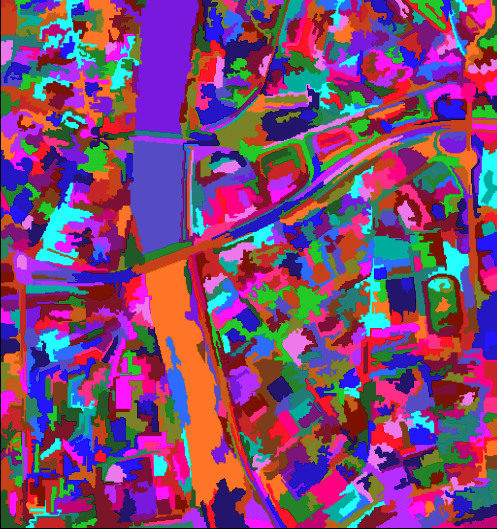
\includegraphics[width=0.6\textwidth]{../Art/MonteverdiImages/seg3.png}
  \itkcaption[Monteverdi seg3]{Optimally colored labels image.}
  \label{fig:seg3}
\end{figure}

Now it should be nice to superimpose this colorization with the original image to assess the quality of the segmentation.
\mont provides the user a very simple way to do it. Once the two images are loaded in \mont and that the original image is placed on the top of the stack, 
the user just has to select the translucency layer effect and set the size of the exploration circle to convenience.
The figure below (~\ref{fig:seg4}) shows the result of such colorization. We encourage the reader to test the other layer effects.

\begin{figure}[!h] 
  \center
  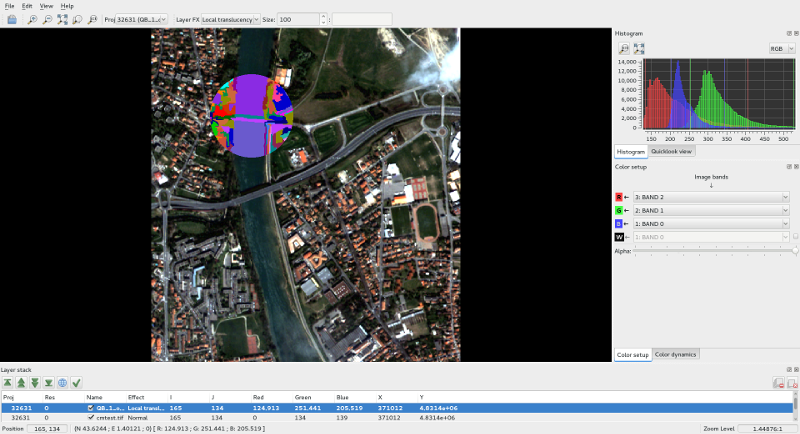
\includegraphics[width=0.95\textwidth]{../Art/MonteverdiImages/seg4.png}
  \itkcaption[Monteverdi seg4]{Nice layer effect, local translucency, to ease the comparison between the original image and its segmentation.}
  \label{fig:seg4}
\end{figure}

\subsection{Polarimetry}\label{ssec:monpolar}
In this example, we are going to use three applications : 
\begin{itemize}
\item the first one is SARDecompositions. This application is used to compute the HaA decomposition. It takes as inputs three complex channels from bands HH HV and VV.
\item the second one is SplitImage. Indeed, the previous application had produced an output image made up of three channels, H a and A, and we wish to focuse on the H parameter (entropy). 
So we let this application split this image into three one-band-images.
\item the last one is ColorMapping. The entropy image has values ranging from 0 to 1, and they can be easily displayed by \mont. But since we have a nice visualizing tool in hand, we wish we could go a little bit further.
Here comes the application ColorMapping. It is going to be used with the following parameter settings:
\begin{itemize}
\item method = continous. This parameters tells the application to use a gradient of colors to represent the entropy image.
\item method.continuous.lut = hot. We specify here the kind of gradient to be used : low values in black, high ones in white, and intermediate ones in red/orange/yellow...
\item method.continuous.min = 0 and method.continuous.max = 1. Here, the gradient of colors must be adjusted to the dynamic of the entropy image (note: it is theoretically known that in HaA decomposition, H ranges from 0 to 1. Generally speaking, the histogram of \mont can also be used for this purpose).
\end{itemize}
\end{itemize}

In the figure below (~\ref{fig:pol1}), we show the obtained result, with the local contrast layer effect.

\begin{figure}[!h] 
  \center
  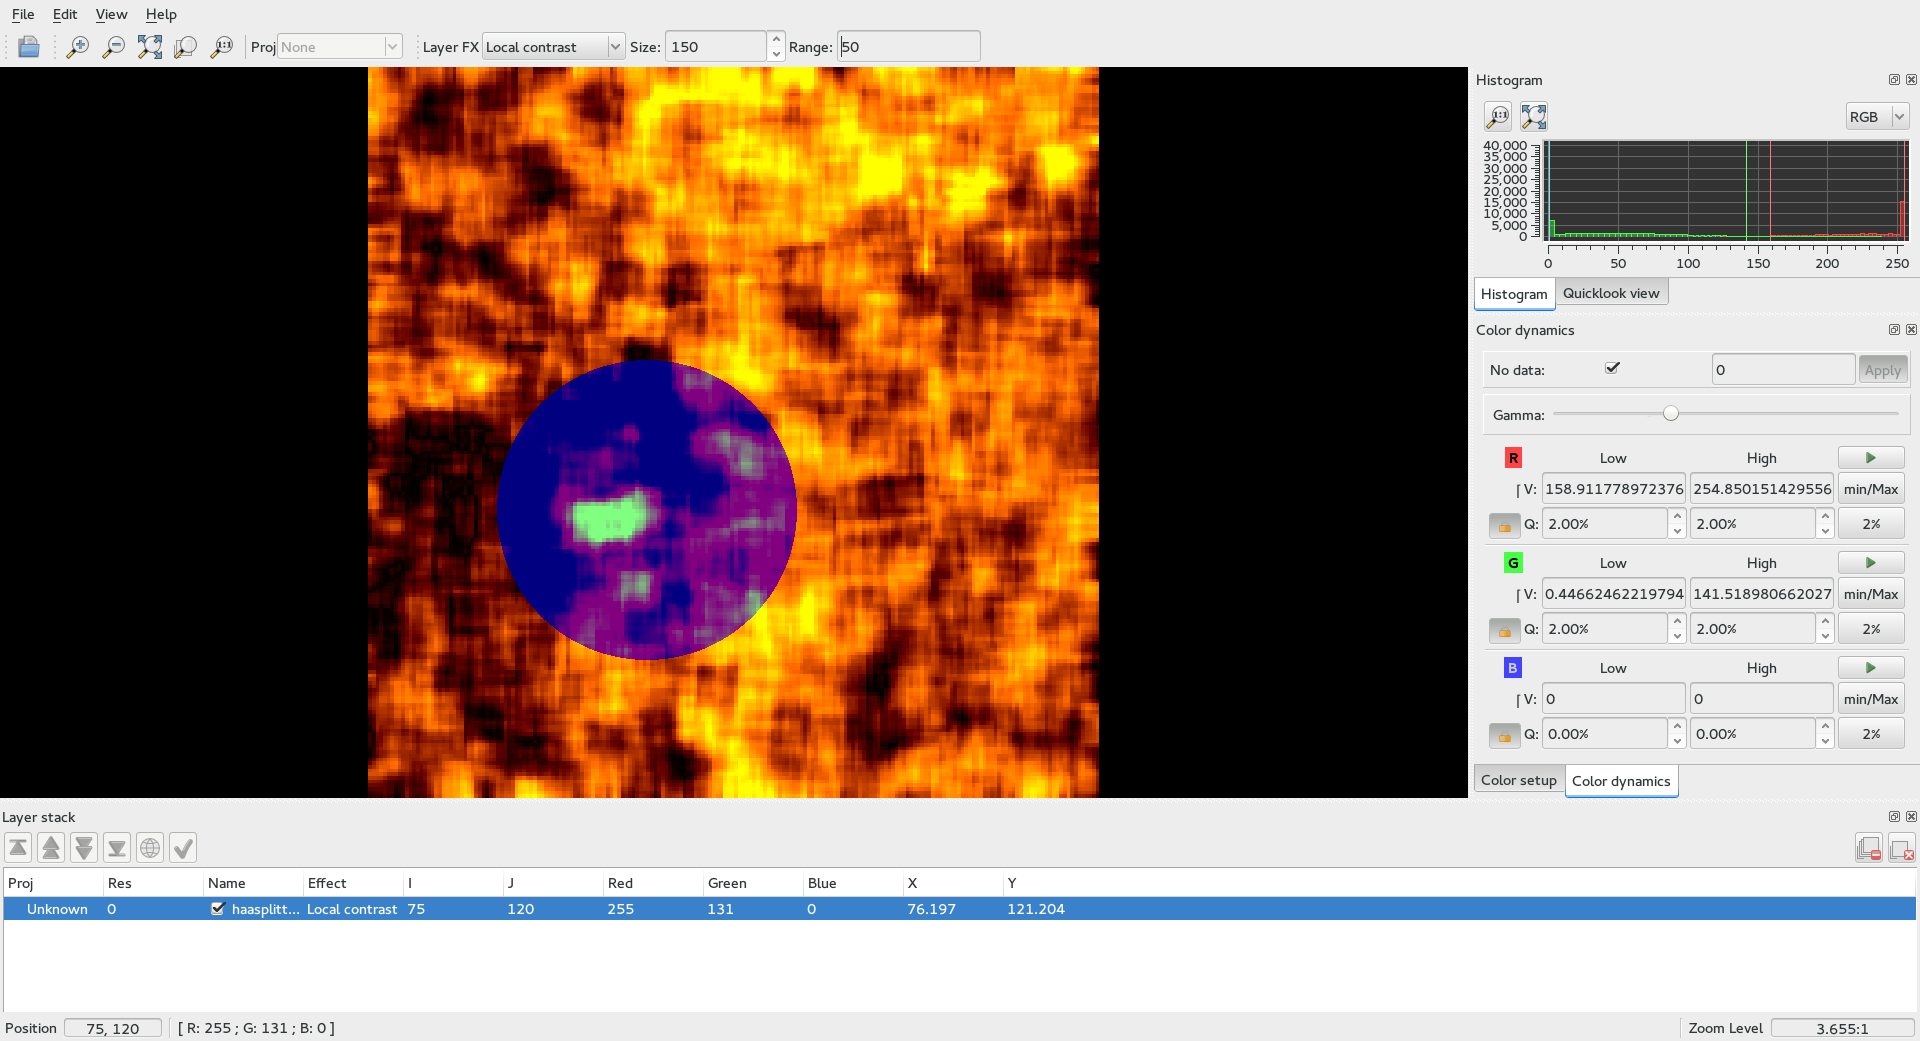
\includegraphics[width=0.95\textwidth]{../Art/MonteverdiImages/pol1.png}
  \itkcaption[Monteverdi pol1]{Entropy image represented in temperature colors; layer effet : local constrast.}
  \label{fig:pol1}
\end{figure}


\subsection{Pansharpening}\label{ssec:monpansh}
Finally, let's try a last example with the Pansharpening application (launch it with shortcut CTRL+A).
The fields are quite easy to fill in : this application needs a panchromatic image, a XS image, and an output image.
These images are represented in the figures below (~\ref{fig:ps12} and ~\ref{fig:ps3}):

\begin{figure}[!h] 
  \center
  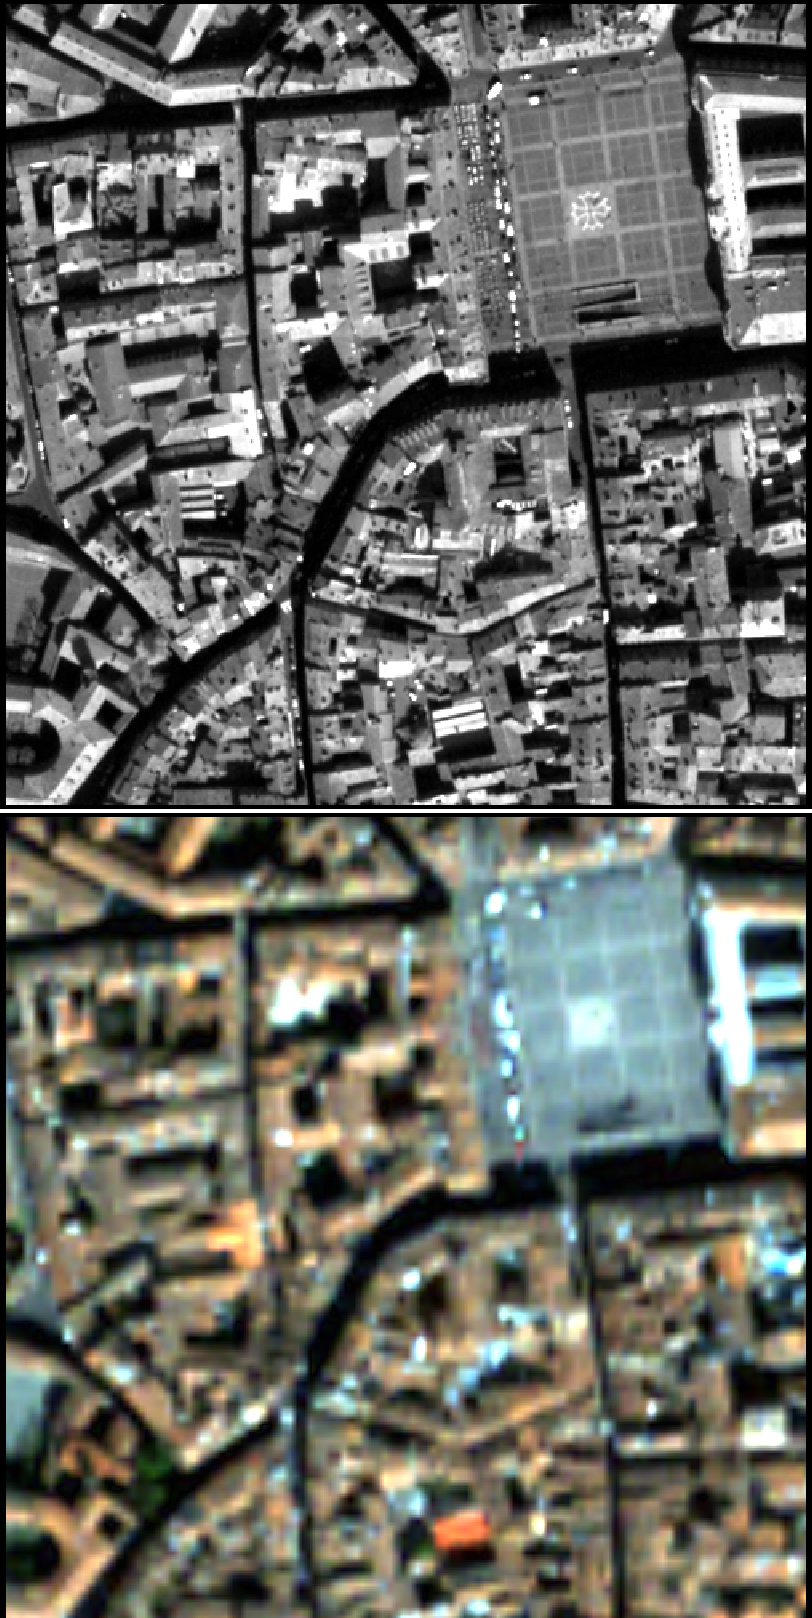
\includegraphics[width=0.6\textwidth]{../Art/MonteverdiImages/ps1-2.png}
  \itkcaption[Monteverdi ps12]{Panchromatic and XS images.}
  \label{fig:ps12}
\end{figure}

\begin{figure}[!h] 
  \center
  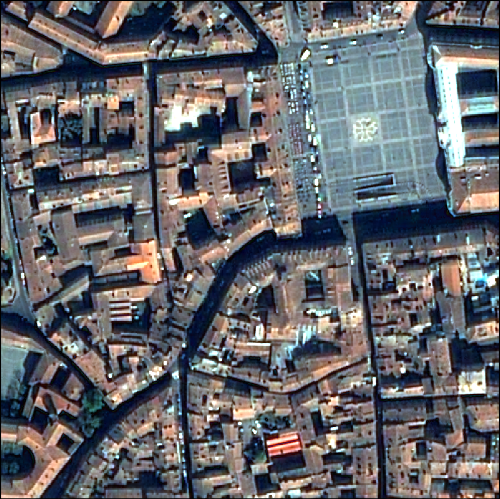
\includegraphics[width=0.6\textwidth]{../Art/MonteverdiImages/ps3.png}
  \itkcaption[Monteverdi ps3]{Pansharpened image.}
  \label{fig:ps3}
\end{figure}

Now, in order to inspect the result properly, these three images are loaded in \mont.
The pansharpened image is placed to the top of the stack layer, and different layer effects are applied to it :
\begin{itemize}
\item in figure ~\ref{fig:ps4} : chessboard effect, to compare the result with the XS image.
\item in figure ~\ref{fig:ps5} : translucency effect, to compare the result with the panchromatic image.
\end{itemize}

\begin{figure}[!h] 
  \center
  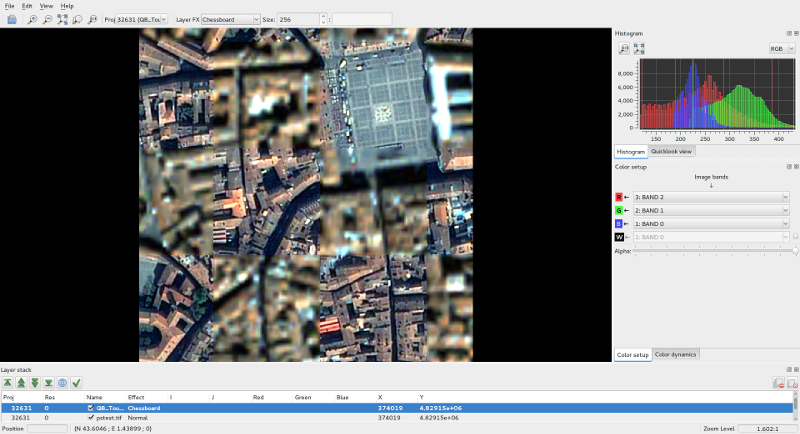
\includegraphics[width=0.95\textwidth]{../Art/MonteverdiImages/ps4.png}
  \itkcaption[Monteverdi ps4]{XS image with panchromatic image; chessboard layer effect.}
  \label{fig:ps4}
\end{figure}

\begin{figure}[!h] 
  \center
  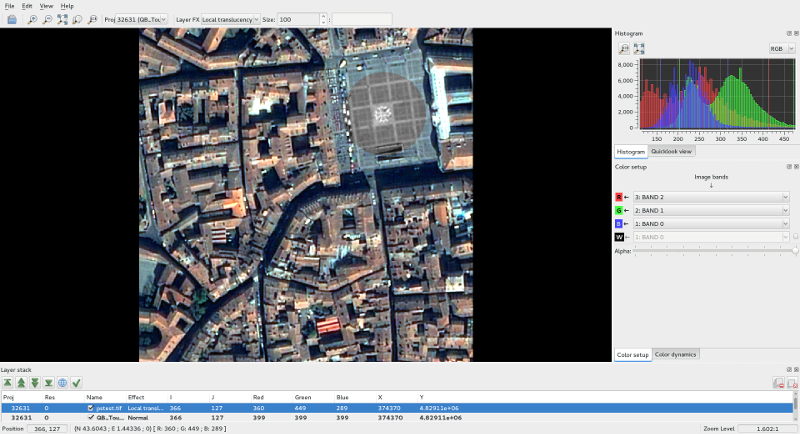
\includegraphics[width=0.95\textwidth]{../Art/MonteverdiImages/ps5.png}
  \itkcaption[Monteverdi ps5]{Pansharpened image with panchromatic image; translucency layer effect (see the Capitol Square at the top right corner).}
  \label{fig:ps5}
\end{figure}


\subsection{Conclusion}\label{ssec:moncon}
The images used in this documentation can be found in the OTB-Data repository (https://git.orfeo-toolbox.org/otb-data.git):
\begin{itemize}
\item in OTB-Data/Input : 
\begin{itemize}
\item QB\_TOULOUSE\_MUL\_Extract\_500\_500.tif and QB\_Toulouse\_Ortho\_XS\_ROI\_170x230.tif (GUI presentation)
\item RSAT\_imagery\_HH.tif RSAT\_imagery\_HV.tif RSAT\_imagery\_VV.tif (polarimetry example)
\item QB\_Toulouse\_Ortho\_PAN.tif QB\_Toulouse\_Ortho\_XS.tif (pansharpening example)
\end{itemize}

\item in OTB-Data/Input/mv2-test : QB\_1\_ortho.tif
\end{itemize}
